\documentclass[11pt, norsk]{article}
%\usepackage[latin1]{inputenc}
\usepackage[T1]{fontenc}
\usepackage[utf8]{inputenc}
\usepackage[norsk]{babel}   % S P R A A K


% \usepackage{graphicx}    % postscript graphics
\usepackage{amssymb, amsmath, amsthm, amssymb} % symboler, osv
\usepackage{mathrsfs}
\usepackage{url}
\usepackage{thmtools}
\usepackage{enumerate}  % lister $  
\usepackage{float}
\usepackage{tikz}
\usetikzlibrary{calc}
\usepackage[all]{xy}   % for comm.diagram
\usepackage{wrapfig} % for float right
\usepackage{hyperref}
\usepackage{mystyle} % stilfilen      


\begin{document}
\title{Oppgaver MAT2500}
\author{Fredrik Meyer}
\maketitle 

\begin{oppg}
La $\{p_1,\cdots,p_n\}$ være hjørnene til en regulær $n$-kant med senter i origo. Vis at definisjonen av \emph{tyngdepunktet} som 
$$T := \frac 1n \sum_{i=1}^n p_i $$
``stemmer''. Det vil, si, vis at $T= \vec 0$, origo.
\end{oppg}
\begin{losn}
Tenk på $E^2=\R^2$ som det komplekse planet, $\C$. Da kan vi identifisere en hjørnene til en regulær $n$-kant med enhetsrøttene $$p_i = e^{\frac{2\pi i k}{n}}$$ for $k=1,2,\ldots,n$.

La $z = e^{\frac{2 \pi i}{n}}$ være $p_1$. Da ser vi at $p_k=z^k$. Dermed er
\[
T = \frac 1n \left( z+z^2+\cdots+z^n \right) = \frac zn (1 + \cdots + z^{n-1}) = \frac zn \frac {z^n-1}{z-1}.
\]
Men $z^n = e^{2\pi i}=1$, så $T=0$, akkurat som vi ønsket.
\end{losn}

\begin{oppg}
  La $M= \{ m \vec x + n \vec y \mid m,n \in \Z \}=\vec x \Z \oplus \vec y \Z$ være gitteret utspent av vektorene $\vec x$ og $\vec y$. La $D$ være det tilhørende Dirichlet-området. Tegn $D$ og beskriv symmetrigruppa til $D$.
  \begin{enumerate}[a)]
  \item Når $\vec x = (1,0)$ og $\vec y = (0,1)$.
  \end{enumerate}
\end{oppg}
\begin{losn}
  \begin{enumerate}[a)]
  \item Vi starter med å tegne standardparallellogrammet. Dette består av seks trekanter, og vi skal finne omsentrene til disse trekantene\footnote{Husk at et \emph{omsenteret} til en trekant er skjæringspunktet til midtnormalene.}. I dette tilfellet sammenfaller flere av omsentrene, og vi får et kvadrat. Se Figur 1, hvor Dirichlet-området er merket i gult. Dermed blir symmetrigruppen $D_4$, firkantgruppen.
\begin{figure}[h]
\begin{center}
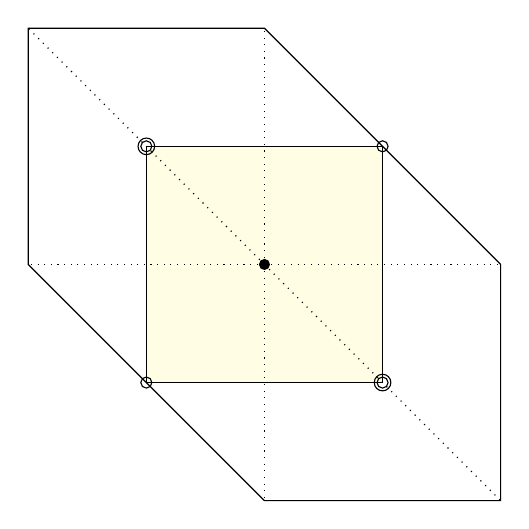
\begin{tikzpicture}
\coordinate (A) at (0,0);
\coordinate (B) at (3,0);
\coordinate (C) at (-3,0);
\coordinate (D) at (0,-3);
\coordinate (E) at (3,-3);
\coordinate (F) at (-3,3);
\coordinate (G) at (0,3);
\coordinate (x1) at (1.5,1.5);
\coordinate (x2) at (-1.5,1.5);
\coordinate (x3) at (-1.5,1.5);
\coordinate (x4) at (-1.5,-1.5);
\coordinate (x5) at (1.5,-1.5);
\coordinate (x6) at (1.5,-1.5);

\draw[thin, draw=black, fill=yellow, fill opacity = 0.1]
     (x1) -- (x2) -- (x4)  -- (x5) -- cycle;

\draw (x1) circle (2pt);
\draw (x2) circle (2pt);
\draw (x3) circle (3pt);
\draw (x4) circle (2pt);
\draw (x5) circle (2pt);
\draw (x6) circle (3pt);

\fill (A) circle (2pt);
\draw (B) --(E) -- (D) -- (C)-- (F)-- (G) --(B);
\draw[dotted] (A) -- (B);
\draw[dotted] (A) -- (C);
\draw[dotted] (A) -- (D);
\draw[dotted] (A) -- (E);
\draw[dotted] (A) -- (F);
\draw[dotted] (A) -- (G);
\end{tikzpicture}
\end{center}
\caption{Dirichlet-området i a).}
\end{figure}

\item I dette tilfellet er $\vec x = (1,0)$ og $\vec y = \frac 12 (1, \sqrt{3})$. Trekanten $OAB$ er da en likesidet trekant, så Dirichlet-området blir en regulær sekskant. Symmetrigruppen blir da $D_6$. 
\item Nå er $\vec x=(1,0)$ og $\vec y = \frac 12 (1,2)$. Se Figur 2 for Dirichlet-området. Vi får en sekskant, men den er ikke regulær, så vi har ingen rotasjonssymmetri. Men vi ser at vi kan speile i $x$-aksen og i $y$-aksen. Sammensetningen av disse to speilingene blir en rotasjon på $180^\circ$. Så til sammen har vi fire symmetrier, og vi kan kalle gruppa for $\Z/2 \times \Z/2$.
\begin{figure}[h]
\begin{center}
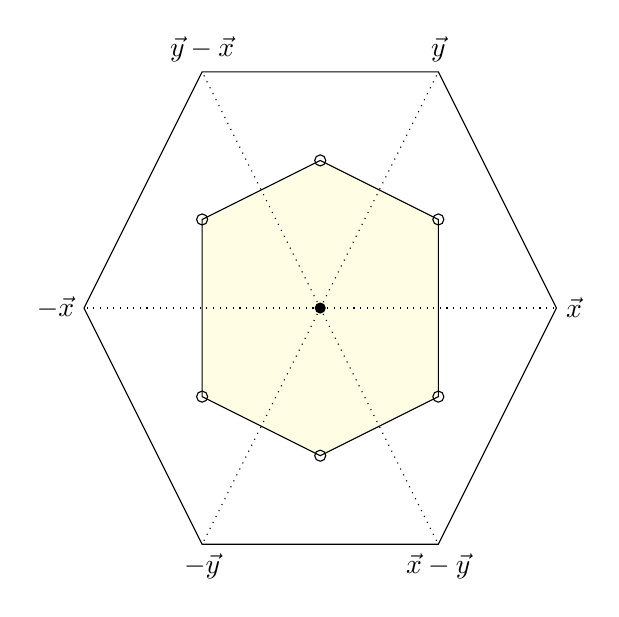
\begin{tikzpicture}
\coordinate (A) at (0,0);
\coordinate (B) at (3,0); % x
\coordinate (C) at (-3,0); % -x
\coordinate (D) at (-3/2,-3); % -y
\coordinate (E) at (3/2,-3); % x-y
\coordinate (F) at (-3/2,3); % y-x
\coordinate (G) at (3/2,3); %% y
\coordinate (x1) at (1.5,9/8);
\coordinate (x2) at (0,15/8);
\coordinate (x3) at (-1.5,9/8);
\coordinate (x4) at (-1.5,-9/8);
\coordinate (x5) at (0,-15/8);
\coordinate (x6) at (1.5,-9/8);

\draw[thin, draw=black, fill=yellow, fill opacity = 0.1]
     (x1) -- (x2) -- (x3) -- (x4)  -- (x5) -- (x6) -- cycle;

\draw (x1) circle (2pt);
\draw (x2) circle (2pt);
\draw (x3) circle (2pt);
\draw (x4) circle (2pt);
\draw (x5) circle (2pt);
\draw (x6) circle (2pt);

\fill (A) circle (2pt);
\draw (B) --(E) -- (D) -- (C)-- (F)-- (G) --(B);
\draw[dotted] (A) -- (B) node[right] {$\vec x$};
\draw[dotted] (A) -- (C) node[left] {$-\vec x$};
\draw[dotted] (A) -- (D) node[below] {$-\vec y$};
\draw[dotted] (A) -- (E) node[below] {$\vec x - \vec y$};
\draw[dotted] (A) -- (F) node[above] {$\vec y - \vec x$};
\draw[dotted] (A) -- (G) node[above]{$\vec y$};
\end{tikzpicture}
\end{center}
\caption{Dirichlet-området i c).}
\end{figure}
  \end{enumerate}
\end{losn}

\begin{oppg}
Vis at en diskret undergruppe av $SO(2)$ er endelig.
\end{oppg}
\begin{losn}
Husk at $SO(2)$ er gruppen av ortogonale operatorer på $\R^2$. Konkret er dette mengden av ortogonale $2 \times 2$-matriser. Disse kan alle dekomponeres som $M=SM_\theta$, der $S$ er matrisen til speiling om $x$-aksen og $M_\theta$ er en rotasjon på $\theta$ grader om origo.

Husk at en undergruppe $G$ av $SO(2)$ er \emph{diskret} hvis det finnes en $\epsilon > 0$ slik at for hver rotasjon $M_\theta$ i $G$, så er $\lvert \theta \rvert \geq \epsilon$ (om $\theta \neq 0$). På mer forståelig norsk betyr dette at alle rotasjonene i $G$ roterer mer enn $\epsilon$ grader.

Nå påstår jeg at dette impliserer at om $M_\theta,M_\varphi$ er to rotasjoner i $G$, så er $\lvert\theta - \varphi\rvert \geq \epsilon$. Siden $G$ er en gruppe, er også $M_\varphi^{-1} \in G$, og følgelig også $M_{\theta}M_{\varphi}^{-1} = M_\theta M_{-\varphi}=M_{\theta-\varphi}$. Men siden $G$ er diskret, følger det at $\lvert \theta - \varphi\rvert \geq \epsilon$.

Dermed har alle rotasjonene i $G$ en avstand på større enn $\epsilon$, noe som betyr at vi maksimalt kan ha $\frac{2\pi}{\epsilon}$ rotasjoner i $G$. Så en diskret undergruppe av $SO(2)$ kan bare inneholde endelig mange rotasjoner, og siden $SM_\theta = M_{-\theta}S$, følger det at maksimal størrelse på $G$ er $\frac{4\pi}{\epsilon}$ (ved å putte inn maksimalt antall speilinger).
\end{losn}

\begin{oppg}
 Hvis $G \subset Isom_2$ er en diskret undergruppe og rangen til $L_G$ er $2$, vis at $D_G$, Dirichlet-området, er et fundamentalområde for $L_G$.
\end{oppg}

\begin{losn}
For å vise at $D_G$ er et fundamentalområde må vi vise to ting: Det ene er at $E^2=\R^2$ er dekket av translasjoner/rotasjoner av $D_G$: $E^2 = \cup_{g \in G} g(D_G)$. Det andre er at når $g \neq h$, så er det indre av $g(D) \cap h(D)$ tom.

Først: Kall vektorene i gitteret for $\vec x$ og $\vec y$. La $\vec a = (a,b) \in \R^2$. Siden $\vec x,\vec y$ utgjør en basis, kan vi skrive $\vec a = r_1 \vec x + r_2 \vec y$ for noen $r_1,r_2 \in \R$. Nå, skriv $r_1$ og $r_2$ som en sum av heltall pluss et tall i intervallet $[-\frac 12,\frac 12)$ (dette kan vi alltid gjøre, og til og med unikt), altså som $r_1=n_1 + s_1, r_2=n_2+s_2$, der $n_1,n_2$ er heltall, og $s_1,s_2$ er i intervallet over. Da er $\vec x = t_{n_1 \vec x}t_{n_2 \vec y}(s_1 \vec x + s_2 \vec y)$.

Nå påstår jeg at $s_1 \vec x + s_2 \vec y$ ligger innenfor Dirichlet-området til $G$. Men å ligge innenfor Dirichlet-området er det samme som å ligge innenfor alle midtnormalene til trekantene i fundamentalheksagonet. Så om $s_1 \geq 0$ og $s_2 \geq 0$, er vi automatisk i den første trekanten. Anta nå $s_1 < 0$ og $s_2 > 0$. Om $s_1+s_2 < \frac 12$, kan vi skrive
\[
s_1 \vec x + s_2 \vec y = s_1 \vec x -s_1 \vec y +s_1 \vec y + s_2 \vec y = (-s_1)(\vec y - \vec x) + (s_1+s_2) \vec y.
\]
Dermed er $s_1 \vec x + s_2 \vec y$ i den øverste trekanten. Om $s_1 + s_2 > \frac 12$ kan vi skrive
\[
s_1 \vec x + s_2 \vec y = (-s_1-s_1)(-\vec x) + s_2(\vec y- \vec x).
\]
Da er $s_1 \vec x + s_2 \vec y$ i den øvre, venstre trekanten.

Repeter samme argumenter for $s_2 < 0$, og konkluder med at hvert element $\vec a \in \R^2$ kan skrives som et element i $D_G$, pluss heltallskombinasjoner av $\vec x,\vec y$. Dette er det samme som å si at $\R^2 = \cup_{g \in G} g(D_G)$.

Det andre kravet for å være et fundamentalområde var at om $g \neq h$, så hadde vi at $g(D_G) \cap h(D_G)$ ikke hadde noe indre. Men dette er klart: det ``verste'' som kan skje er at $g(D_G)$ og $h(D_G)$ er naboer, men da snitter de kun i randen.
\end{losn}

PS: Til slutt en formel jeg måtte bruke for å lage noen av diagrammene i løsningsforslaget. Vi skulle finne omsenteret til en trekant. Anta ene hjørnet er origo, og andre er $(a,b)$, og tredje er $(c,d)$. Da kan vi regne ut at omsenteret har koordinater:
\[
\frac{1}{2(bc-ad)} \left( a^2d-d^2b+b^2d-c^2b, a^2c + b^2c - ac^2- ad^2 \right)
\]
Hvordan jeg fant denne formelen: la $\ell$ være linjen $\frac 12 \vec a + t \vec a^\perp$ (altså linjen som står ortogonalt på $\vec a$ og går ut fra midtpunktet). La $\ell^\prime$ være den tilsvarende linjen for $\vec b$. Da kan man regne ut skjæringspunktet mellom disse linjene, og dette er omsenteret (engelsk \emph{circumcenter}).
\end{document}
 
